\section{Graphen}

Graphen können in Latex direkt mit Hilfe der Pakete \verb+tikz+ und \verb+pgfplots+ (\url{http://www.ctan.org/pkg/pgfplots}) gemacht werden. Wie diese auszusehen haben ist dabei nicht so universell definiert wie bei den Tabellen. In Bild \ref{fig:example-graph} ist ein Beispiel für einen Plot dargestellt, wie er hier am Lehrstuhl gewünscht wird.

\begin{figure}[H]%
    \centering
    % do not externalise this picture
    \tikzset{external/export next=false}
    
    \begin{tikzpicture}
        \begin{axis}[
            ymin=-1.5, ymax=1.5,
            xmin=0, xmax=15,
            width=15cm, height=10cm,
            ylabel={Speed, \unitfrac{m}{s}},
            xlabel={Time, \unit{s}},
            ignore legend
            ]
        
            \addplot+[only marks, mark=x, mark size=3, forget plot] table[x=time, y=value, col sep=semicolon] {data/measurements-data.csv};
            \addlegendentry{Messdaten Sinus}
            \label{graph:measurement-sine}
            \addplot+[mark=none] table[x=time, y=value, col sep=semicolon] {data/simulation-data.csv};
            \addlegendentry{Simulationsdaten Sinus}
            \label{graph:simulation-sine}
            
            \addplot+[simulation-plot] plot[domain=0:15, samples=500, smooth] {cos(x/pi*180)}; 
            \label{graph:simulation-cosine}
        \end{axis}
    \end{tikzpicture}
    
    
    \caption{Beispielgraph. Dargestellt sind die Messdaten der Sinuskurve (\protect\plotref{graph:measurement-sine}), die zugehörige Simulation (\protect\plotref{graph:simulation-sine}) sowie eine Simulation, die eine Alternative konfiguration wiedergibt (\protect\plotref{graph:simulation-cosine})}%
    \label{fig:example-graph}%
\end{figure}

Generell haben Graphen in schriftlichen Arbeiten keinen Titel. Achsenbeschriftungen sind zwingend erforderlich (vgl. Abbildung \ref{fig:label-your-axes-xkcd}) und müssen mit einer Einheit versehen werden. Die Beschriftung der Achsen und der Zahlen sollte nicht zu klein sein (Schriftgröße mind. 14pt, in latex \verb+\normalsize+).

\begin{figure}[H]%
    \centering

    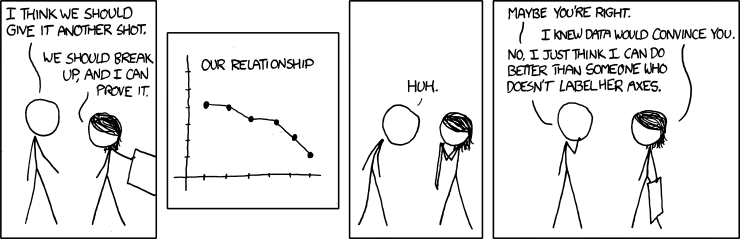
\includegraphics[width=0.8\columnwidth]{images/examples/axes-xkcd}%
    \caption{"`Convincing"', \href{http://xkcd.com/833/}{xkcd.com/833}}%
    \label{fig:label-your-axes-xkcd}%
\end{figure}

Weiterhin gilt:

\begin{itemize}
	\item Um den Graph herum ist ein schwarzer, ertwas dickerer Rahmen zu ziehen (Latex/pgfplots: \verb+axis line style={thick}+).
    \item Hilflinien sind in dünn und hell bei den Hauptachsenmarkierungen waagrecht und senkrecht zu zeichnen. Die Linien können dabei durchgezogen oder gestrichelt sein. In Latex/Pgfplots wird das gezeigte Ergebnis durch \verb+grid=major+ und \verb+grid style={help lines, dashed, thin}+ erreicht.
    \item Messwerte werden durch einzelne Markierungen dargestellt, während simulierte Daten durchgängige Linien erhalten. Die Farben sollten so gewählt werden, dass der Ausdruck in schwarz/weiss erkennbar ist. Zusammengehörige Mess-/Simulationsdaten können dabei die gleiche Farbe erhalten. Für Messdaten kann die s/w--Eindeutigkeit durch Wechsel des Symbols erleichtert werden.
    \item Am Lehrstuhl wird die Legende nicht im Graph dargestellt, sondern in der Bildunterschrift. Dies kann bei pgfplots über das setzen von \verb+\label+s und Referenezierung über \verb+\protect\ref+ erreicht werden. \textcolor[rgb]{0.55,0,0}{Achtung}: Bei Nutzung von \verb+\tikzexternalize+ kann dies zu Fehlern führen! Hierbei muss die Externalisierung für die Refernez deaktiviert werden. Dazu kann auch das in dieser Vorlage definierte \verb+\plotref+ genutzt werden.
\end{itemize}

Vereinfacht können die generellen Darstellungseigenschaften eines Graphen über den folgenden Eintrag in der Präambel des Dokuments definiert werden, wie es in dieser Vorlage (\verb+elements/preamble.options.tex+) bereits umgesetzt ist:

\begin{Verbatim}[fontsize=\small,gobble=4]
    \pgfplotsset{
        every axis/.append style={
            grid=major,
            grid style={help lines, dashed, thin},
            axis line style={thick},
            title style={font=\large\bfseries, text centered},
            label style={font=\normalsize},
            tick label style={font=\normalsize},
        }
    }
\end{Verbatim}

Um die Darstellung der Simuations- und Messdaten zu vereinfachen, existieren in dieser Vorlage weiterhin Kürzel, welche bei Plots genutzt werden können um die generelle Darstellung zu vereinfachen (\verb+elements/preamble.tweaks.tex+). Für eine genaue Bedeutung der jeweiligen Befehle möchte ich auf das \href{http://mirrors.ctan.org/graphics/pgf/contrib/pgfplots/doc/pgfplots.pdf}{pgfplots-Manual} verweisen. Ein Beispiel für de Anwendung findet sich im Code von Graph \ref{fig:example-graph}. 

\begin{Verbatim}[fontsize=\small,gobble=4]
    \pgfplotsset{
        simulation-plot/.style = {
          each nth point=10, filter discard warning=false,
          mark=none, 
          x=Time,
          thick,
          },
        measurements-plot/.style = {
          mark=*, only marks, mark size=2pt, mark options={},
          x=Time,
          forget plot,
          error bars/y dir=both, error bars/y fixed relative=0.05,
          },
    }
\end{Verbatim}

Und --- last but not least --- nochmal der Hinweis:

\begin{figure}[H]%
    \centering
    
    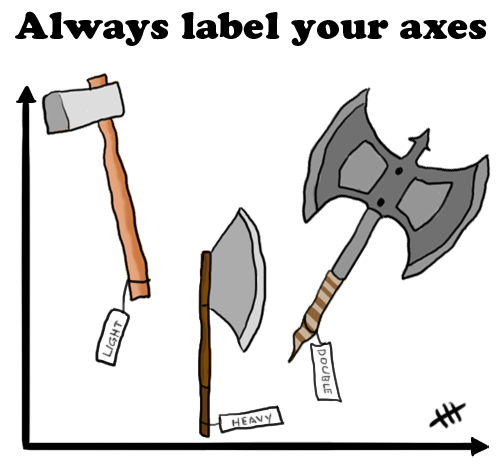
\includegraphics[width=0.4\columnwidth]{images/examples/axes-fluffware}%
    \caption{"`Always label your axes"', Quelle \href{http://fluffware.tumblr.com/post/4580822773/axes}{Fluffware}}%
    \label{fig:label-your-axes-fluffware}%
\end{figure}
